\documentclass[11pt,spanish]{article}

\usepackage{listings}             
\usepackage{anysize} 
\usepackage{graphicx}
\usepackage[spanish]{babel}
\usepackage[utf8]{inputenc}
\usepackage{xcolor}
\usepackage{wrapfig}
\usepackage{amsmath}

\lstset{language=Python}
\marginsize{1cm}{1cm}{2cm}{2cm}
\selectlanguage{spanish}
\lstset{
language=Python,
 backgroundcolor=\color{red!75!green!50!blue!25},
 frame=single,
literate=
  {á}{{\'a}}1 {é}{{\'e}}1 {í}{{\'i}}1 {ó}{{\'o}}1 {ú}{{\'u}}1
  {Á}{{\'A}}1 {É}{{\'E}}1 {Í}{{\'I}}1 {Ó}{{\'O}}1 {Ú}{{\'U}}1
  {à}{{\`a}}1 {è}{{\`e}}1 {ì}{{\`i}}1 {ò}{{\`o}}1 {ù}{{\`u}}1
  {À}{{\`A}}1 {È}{{\'E}}1 {Ì}{{\`I}}1 {Ò}{{\`O}}1 {Ù}{{\`U}}1
  {ä}{{\"a}}1 {ë}{{\"e}}1 {ï}{{\"i}}1 {ö}{{\"o}}1 {ü}{{\"u}}1
  {Ä}{{\"A}}1 {Ë}{{\"E}}1 {Ï}{{\"I}}1 {Ö}{{\"O}}1 {Ü}{{\"U}}1
  {â}{{\^a}}1 {ê}{{\^e}}1 {î}{{\^i}}1 {ô}{{\^o}}1 {û}{{\^u}}1
  {Â}{{\^A}}1 {Ê}{{\^E}}1 {Î}{{\^I}}1 {Ô}{{\^O}}1 {Û}{{\^U}}1
  {œ}{{\oe}}1 {Œ}{{\OE}}1 {æ}{{\ae}}1 {Æ}{{\AE}}1 {ß}{{\ss}}1
  {ű}{{\H{u}}}1 {Ű}{{\H{U}}}1 {ő}{{\H{o}}}1 {Ő}{{\H{O}}}1
  {ç}{{\c c}}1 {Ç}{{\c C}}1 {ø}{{\o}}1 {å}{{\r a}}1 {Å}{{\r A}}1
  {€}{{\EUR}}1 {£}{{\pounds}}1
}


\title{\vspace{-3cm}\begin{flushleft}\textbf{Actividad 4}\end{flushleft}}
\author{\hspace{-9.6cm}\textsc{Andrés Ignacio Rodríguez Mendoza}}
\date{}

\begin{document}

\begin{wrapfigure}{r}{0.2\textwidth}
  \begin{center}
   \vspace{-5.4cm} 
\includegraphics[width=0.15\textwidth]{uni}
  \end{center}
\end{wrapfigure}

\maketitle  
\begin{center}
\rule{\textwidth}{1pt}
\end{center}
\section*{Introducción}

El análisis de regresión es un proceso estadístico para estimar las relaciones entre variables. Ayuda a entender como un valor típico de la variable dependiente cambia cuando cualquiera de las variables independientes es variada, mientras las otra permanecen fijas. Un procedimiento estandar es el de mínimos cuadrados, una solución aproximada a un sistema de ecuaciones que contiene más ecuaciones que incógnitas. La solución es la que minimiza la suma de los cuadrados de los errores hechos en el resultado de cada ecuación.\\ \\
En esta práctica se presenta el ajuste de datos, la aplicación más importante de mínimos cuadrados. El ajuste minimiza la suma de los residuales cuadrados, siendo un residual la diferencia entre un valor observado y el dado por el modelo.\\ \\
El paquete de scipy.optimize provee varios algoritmos de optimización comunmente usados. El módulo contiene a $scipy.optimize.least\_squares$, que resuelve un problema de minimos cuadrados no lineal con fronteras en las variables; y $scipy.optimize.curve\_fit$, wue usa el ajuste de minimos cuadrados no lineal para ajustar una función a los datos. En este código se reemplaza la funcion $scipy.optimize.least\_squares$ por $np.polyfit$, que obtiene los coeficientes de un polinomio $n$, con $n$ igual a $1$ en este caso.

\section*{Código}

\begin{lstlisting} % Start your code-block
import numpy as np
from scipy import optimize
import matplotlib.pyplot as plt



data = np.loadtxt('data.txt')

x=data[:,0].astype(np.int)
y=data[:,1].astype(np.float)


xn=np.linspace(1900,2000,2)

m, c = np.polyfit(x, y, 1)
yn = np.polyval([m, c], xn)

plt.plot(x, y, 'or', label="Datos")
plt.plot(xn, yn, label="Ajuste")
plt.title('Ajuste lineal, temperatura New York')
plt.legend()
plt.show()


data1=np.loadtxt('data1.txt')

x1=data1[:,0].astype(np.int)
y1=data1[:,1].astype(np.float)


def f(x,u,v,w):
    return u*np.exp(-v*x) + w
    
    
popt, pcov = optimize.curve_fit(f, x1, y1)


    
xm=np.linspace(-0,50,1000)

plt.plot(x1, y1, 'or', label="Datos")
plt.plot(xm,f(xm,*popt), label="Ajuste")

plt.title('Ajuste exponencial, presión-altitud')
plt.legend()
plt.show()

\end{lstlisting}

\section*{Gráficas}

\centering


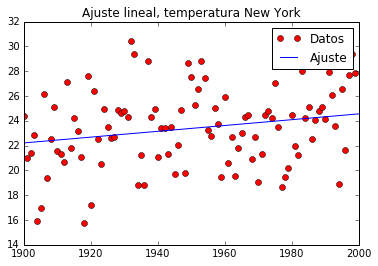
\includegraphics{graph1}\\
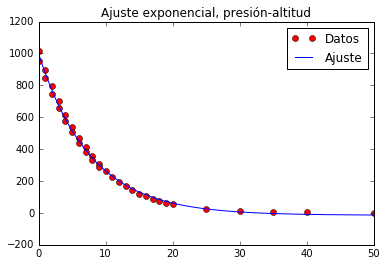
\includegraphics{graph2}\\





\end{document}

